\chapter{Detección de biomarcadores en cáncer de hígado y colon-recto}

\section{Objetivos}

El objetivo general consiste en intentar predecir en base a pocos genes si una enfermedad padece o no cáncer de hígado, o cáncer de colon-recto. Para ello se usarán distintas técnicas de selección de características: mRMR, RF y DA, así como varios algoritmos de clasificación: SVM, RF y kNN.

\section{Metodología}

\subsection{Fuente de datos}

La fuente de los datos es GDC (Genomic Data Commons) Portal, una plataforma web sobre cáncer del Instituto Nacional del Cáncer de Estados Unidos (\textit{National Cancer Institute}) \cite{GDCPortal, NationalCancerInstitute}. GDC Portal fue desarrollado por el Instituto Nacional del Cáncer de Estados Unidos, la Universidad de Chicago, el Instituto de Ontario para la Investigación del Cáncer y la empresa \textit{Leidos Biomedical Research}, y su principal fortaleza reside en la integración y armonización de diversas fuentes heterogéneas, creando así un sistema de información amplio y robusto \cite{Grossman2016}. \\

\newpage
\textbf{\textcolor{red}{Figura XX}}. Diagrama de funcionalidad y utilidad de GDC. Extraído de Grossman et al. \cite{Grossman2016}.
\begin{center}
	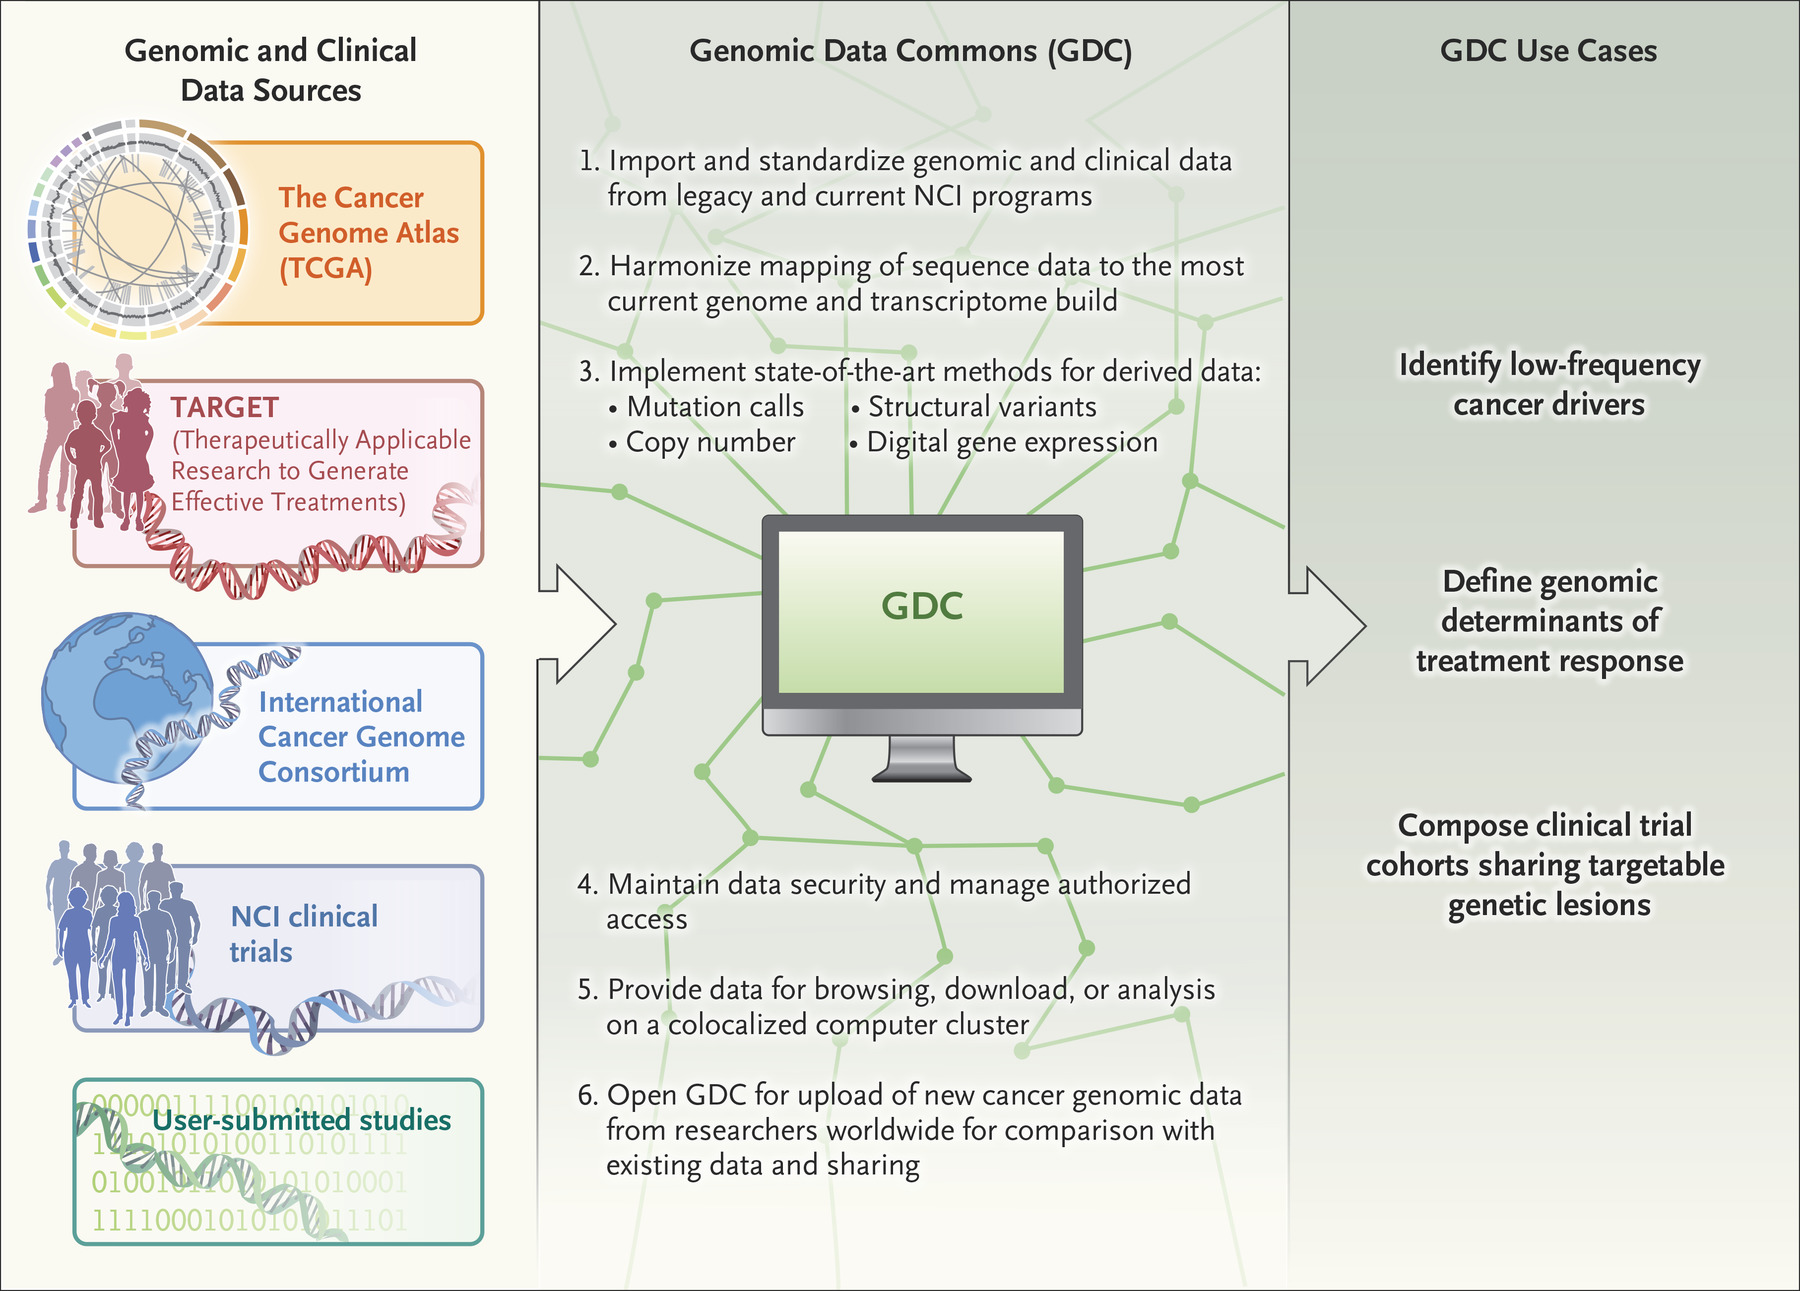
\includegraphics[width=1\textwidth]{figuras/funcionamiento_gdc.jpeg} \\
\end{center}

A día 22 de Junio, GDC Portal contenía información sobre unos 84.000 casos, 23.000 genes y más de 3 millones de mutaciones de genes \cite{GDCPortal}. Algunos de estos datos son abiertos, mientras que para otros es necesario solicitar acceso. La información de la que dispone es muy variada, y se puede distinguir en tres grandes categorías:

\begin{itemize}
	\item Información clínica, como la edad del sujeto, su sexo o el estadio del cáncer del que ha sido diagnosticado.
	\item Información genética y transcriptómica proveniente de diversos proyectos de investigación.
	\item Imágenes de tejidos tumorales y sanos.
\end{itemize} 

Para el presente trabajo se han descargado de GDC Portal todos los datos que cumplen las siguientes condiciones:

\begin{itemize}
	\item Son datos transcriptómicos del programa Cancer Genoma Atlas (TCGA), dirigido por dos organismos estadounidenses: el Instituto Nacional del Cáncer (NCI) y el Instituto Nacional para la Investigación del Genoma Humano (NHGRI) \cite{NationalCancerInstitutea}. 
	\item Contienen información sobre tumores o tejidos sanos de cáncer de hígado, o colon-recto. Se han excluido metástasis y tumores recurrentes.
	\item El tipo de estrategia experimental es RNA-Seq, y el tipo de flujo de trabajo es HTSeq - Counts.
\end{itemize}

Para cáncer de hígado se han descargado datos sobre 462 pacientes, de los cuales 404 tenían cáncer (87,4\%) y 58 estaban sanos (12,6\%).  Para cáncer de colon-recto, se han descargado datos sobre 695 pacientes: 644 con cáncer (92,7\%) y 58 sanos (7,3\%).

\subsection{Análisis}

Para el análisis se ha utilizado el software estadístico \texttt{R} (v.4.0.1) \cite{R} y \{\texttt{KnowSeq}\} (v.1.1.19) \cite{KnowSeq}, paquete de R que ha sido desarrollado por los tutores del presente trabajo, y en el que el autor ha contribuido con pequeñas actualizaciones:

\begin{itemize}
	\item{Mantener los parámetros óptimos de SVM (coste y gamma) y kNN (k) encontrados tras tuning en conjunto de entrenamiento para aplicarlos directamente en el modelo para el conjunto de test}
	\item Pequeñas modificaciones en la documentación de algunas funciones.
\end{itemize}

El paquete está además disponible en Bioconductor, la plataforma de código abierto en R más relevante para el análisis de datos de genómica y transcriptómica \cite{Gentleman2004}.\\

Todo el código de los análisis está disponible la carpeta \texttt{analisis\_higado} del repositorio de GitHub asociado al trabajo \cite{Redondo-Sanchez2020}. Para asegurar la reproducibilidad de los análisis, en el fichero \texttt{session\_info.txt} del repositorio de GitHub \cite{Redondo-Sanchez2020} se muestran todos los paquetes utilizados y sus versiones como resultado de ejecutar \texttt{devtools::session\_info()}.\\

Se utilizan técnicas de visualización de datos para una mejor comprensión de los resultados, utilizando diagramas de Sankey, gráficos de líneas y cajas, y mapas de calor.\\

\section{Características clínicas de los tumores}
 
A continuación se describe la información clínica de aquellas personas diagnosticadas con cáncer. La plataforma GDC Portal permite descargar información clínica sobre los pacientes que tienen casos de cáncer, aunque no sobre los casos sanos \cite{GDCPortal} . 

\subsection{Características clínicas para cáncer de hígado}

En la Tabla 9 se muestra  la distribución de casos de cáncer de hígado según algunas variables de interés. Los casos se recogieron entre los años 1995 y 2013, con el 67,6\% de los casos recogidos entre los años 2010 y 2013. La mayoría de los casos son hombres (65,3\%) y están diagnosticados en estadios iniciales (70,3\% en estadios I y II). La edad media de diagnóstico es de 60,1 años (mediana: 61,7 años), con un rango de edad que comprende de los 16 a los 87 años. Más de la mitad de los casos son blancos (52,5\%), que es la raza más común seguida por asiáticos (39,9\%) y negros o afroamericanos (4,7\%). Aproximadamente dos de cada tres personas estaban vivas en el momento del último contacto realizado (63,6\%).\\

\newpage
\textbf{Tabla 9}. Características clínicas de los casos de cáncer de hígado. Distribución de casos y porcentaje según sexo, grupo de edad, estadio, raza y estado vital.

\begin{table}[H]
	\centering
	\begin{tabular}{rc}
		\cline{2-2}
		\multicolumn{1}{l}{}                           & \multicolumn{1}{c}{\textbf{Número de casos (Porcentaje)}} \\ \hline
		\multicolumn{1}{l}{\textbf{Total}} & 404 (100\%)                                      \\ \hline
		\multicolumn{1}{l}{\textbf{Sexo}}              &                                                  \\
		Hombre                                         & 264 (65,3\%)                                     \\
		Mujer                                          & 140 (34,7\%)                                     \\ \hline
		\multicolumn{1}{l}{\textbf{Grupo de edad}}     &                                                  \\
		$\leq$40 años                                      & 34 (8,4\%)                                       \\
		41-50 años                                     & 40 (9,9\%)                                       \\
		51-60 años                                     & 106 (26,2\%)                                     \\
		61-70 años                                     & 127 (31,4\%)                                     \\
		71-80 años                                     & 77 (19,1\%)                                      \\
		$>$80 años                                       & 16 (4,0\%)                                         \\
		Desconocido                                    & 4 (1,0\%)                                          \\ \hline
		\multicolumn{1}{l}{\textbf{Estadio}}           &                                                  \\
		Estadio I                                      & 189 (46,8\%)                                     \\
		Estadio II                                     & 95 (23,5\%)                                      \\
		Estadio III                                    & 82 (20,3\%)                                      \\
		Estadio IV                                     & 7 (1,7\%)                                        \\
		Desconocido                                    & 31 (7,7\%)                                       \\ \hline
		\multicolumn{1}{l}{\textbf{Raza}}              &                                                  \\
		Blanco                                         & 212 (52,5\%)                                     \\
		Asiático                                       & 161 (39,9\%)                                     \\
		Negro o afroamericano                          & 19 (4,7\%)                                       \\
		Desconocido                                    & 10 (2,5\%)                                       \\
		Indio americano o nativo de Alaska             & 2 (0,5\%)                                        \\ \hline
		\multicolumn{1}{l}{\textbf{Estado vital}}      &                                                  \\ 
		Vivo                                           & 257 (63,6\%)                                     \\
		Fallecido                                         & 146 (36,1\%)                                     \\
		Desconocido                                    & 1 (0,2\%)                                        \\ \hline
	\end{tabular}
\end{table}

En la Tabla 10 se muestran tablas de contingencia del estado vital según sexo, grupo de edad y estadio. Se han realizado pruebas de chi cuadrado ($\chi^2$) \cite{Pearson1900} para evaluar la independencia o no del estado vital con respecto a las distintas variables, aplicando la corrección de Yates \cite{Yates1934} cuando fue necesario.\\

El código completo del análisis se muestra en el fichero \texttt{analisis\_higado/\linebreak01\_analisis\_datos\_clinicos.R} del repositorio de GitHub asociado al trabajo \cite{Redondo-Sanchez2020}.\\

\textbf{Tabla 10}. Características clínicas de los casos de cáncer de hígado. Distribución de  estado vital según sexo, grupo de edad y estadio.

\begin{table}[H]
	\centering
	\begin{tabular}{rrrc}
		\cline{2-4}
		\multicolumn{1}{l}{}                           & \multicolumn{1}{c}{\textbf{Vivos}} & \multicolumn{1}{c}{\textbf{Fallecidos}} & \multicolumn{1}{l}{\textbf{p-valor}} \\ \hline
		\multicolumn{1}{l}{\textbf{Número de casos}} & \multicolumn{1}{c}{257}            & \multicolumn{1}{c}{146}     & \multicolumn{1}{l}{}                     \\ \hline
		\multicolumn{1}{l}{\textbf{Sexo}}              &                           &                             & 0,033                                    \\
		Hombre                                         & 178 (67,7\%)              & 85 (32,3\%)                 &                                          \\
		Mujer                                          & 79 (83,2\%)               & 16 (16,8\%)                 &                                          \\ \hline
		\multicolumn{1}{l}{\textbf{Grupo de edad}}     &                           &                             & 0,018                                    \\
		$\leq$40 años                                      & 24 (70,6\%)               & 10 (29,4\%)                 &                                          \\
		41-50 años                                     & 27 (67,5\%)               & 13 (32,5\%)                 &                                          \\
		51-60 años                                     & 68 (64,2\%)               & 38 (35,8\%)                 &                                          \\
		61-70 años                                     & 89 (70,6\%)               & 37 (29,4\%)                 &                                          \\
		71-80 años                                     & 42 (54,5\%)               & 35 (45,5\%)                 &                                          \\
		$>$80 años                                   & 5 (31,3\%)                & 11 (68,8\%)                 &                                          \\ \hline
		\multicolumn{1}{l}{\textbf{Estadio}}           &                           &                             & $<$0,001                         \\
		Estadio I                                      & 138 (73,4\%)              & 50 (26,6\%)                 &                                          \\
		Estadio II                                     & 64 (67,4\%)               & 31 (32,6\%)                 &                                          \\
		Estadio III                                    & 39 (47,6\%)               & 43 (52,4\%)                 &                                          \\
		Estadio IV                                     & 3 (42,9\%)                & 4 (57,1\%)                  &                                          \\ \hline
	\end{tabular}
\end{table}

Para las variables con datos faltantes se ha realizado un análisis de casos completos.  La mortalidad entre los casos es el doble en hombres (32,3\%) que en mujeres (16,8\%). La mortalidad aumenta conforme aumenta la edad, desde 29,4\% en menores de 41 años hasta 68,8\% en mayores de 80 años. El estadio es uno de los principales factores pronósticos del cáncer, algo que se refleja en la gran diferencia existente en la supervivencia entre estadios. En los estadios iniciales (I-II) la supervivencia está cerca al 30\% y en los más avanzados (III-IV) más cerca del 55\%. Se detecta una dependencia entre todas las variables consideradas (sexo, grupo de edad y estadio)  y el estado vital, con p-valores $<$0,05 en todos los casos.

\subsection{Características clínicas para cáncer de colon-recto}

En la Tabla 11 se muestra  la distribución de casos de cáncer de colon-recto según algunas variables de interés. Los casos se recogieron entre los años 1998 y 2013, con la mayoría de los casos recogidos entre los años 2007 y 2011. La proporción entre hombres y mujeres es similar (53,1\% y 46,9\% respectivamente), y los estadios más comunes son los intermedios (estadio II: 36,3\% y estadio III: 28,7\%). La edad media de diagnóstico es de 66,7 años (mediana: 68,1 años), con un rango de edad de entre 31 y 90 años. Aproximadamente la mitad de los pacientes son blancos (47,3\%), que es la raza más común seguida por negros o afroamericanos (10,5\%) y asiáticos (2,1\%). Se desconoce la raza del 40,0\% de las personas. Aproximadamente cuatro de cada cinco personas estaban vivas en el momento del último contacto realizado (79,2\%).\\

\newpage
\textbf{Tabla 11}. Características clínicas de los casos de cáncer de colon-recto. Distribución de casos y porcentaje según sexo, grupo de edad, estadio, raza y estado vital.

\begin{table}[H]
		\centering
	\begin{tabular}{rr}
		\cline{2-2}
		\multicolumn{1}{l}{}                       & \multicolumn{1}{c}{\textbf{Número de casos (Porcentaje)}} \\ \hline
		\multicolumn{1}{l}{\textbf{Total}}         & 620 (100\%)                                               \\ \hline
		\multicolumn{1}{l}{\textbf{Sexo}}          &                                                           \\
		Hombre                                     & 329 (53,1\%)                                              \\
		Mujer                                      & 291 (46,9\%)                                              \\ \hline
		\multicolumn{1}{l}{\textbf{Grupo de edad}} &                                                           \\
		$\leq$40 años                                   & 16 (2,6\%)                                                \\
		41-50 años                                 & 59 (9,5\%)                                                \\
		51-60 años                                 & 101 (16,3\%)                                              \\
		61-70 años                                 & 173 (27,9\%)                                              \\
		71-80 años                                 & 171 (27,6\%)                                              \\
		$>$80 años                               & 98 (15,8\%)                                               \\
		Desconocido                                & 2 (0,3\%)                                                 \\ \hline
		\multicolumn{1}{l}{\textbf{Estadio}}       &                                                           \\
		Estadio I                                  & 105 (16,9\%)                                              \\
		Estadio II                                 & 225 (36,3\%)                                              \\
		Estadio III                                & 178 (28,7\%)                                              \\
		Estadio IV                                 & 89 (14,4\%)                                               \\
		Desconocido                                & 23 (3,7\%)                                                \\ \hline
		\multicolumn{1}{l}{\textbf{Raza}}          &                                                           \\
		Blanco                                     & 293 (47,3\%)                                              \\
		Asiático                                   & 13 (2,1\%)                                                \\
		Negro o afroamericano                      & 65 (10,5\%)                                               \\
		Desconocido                                & 248 (40\%)                                                \\
		Indio americano o nativo de Alaska         & 1 (0,2\%)                                                 \\ \hline
		\multicolumn{1}{l}{\textbf{Estado vital}}  &                                                           \\
		Vivo                                       & 491 (79,2\%)                                              \\
		Muerto                                     & 129 (20,8\%)                                              \\ \hline
	\end{tabular}
\end{table}

En la Tabla 12 se muestran tablas de contingencia del estado vital según sexo, grupo de edad y estadio. Se han realizado pruebas de chi cuadrado ($\chi^2$) \cite{Pearson1900} para evaluar la independencia o no del estado vital con respecto a las distintas variables, aplicando la corrección de Yates \cite{Yates1934} cuando fue necesario. El código completo del análisis se muestra en el fichero \texttt{analisis\_cr/01\_analisis\_datos\_clinicos.R} del repositorio de GitHub asociado al trabajo \cite{Redondo-Sanchez2020}.\\

\textbf{Tabla 10}. Características clínicas de los casos de cáncer de colon-recto. Distribución de  estado vital según sexo, grupo de edad y estadio.

\begin{table}[H]
		\centering
	\begin{tabular}{rrrc}
		\cline{2-4}
		\multicolumn{1}{l}{}                           & \multicolumn{1}{c}{\textbf{Vivos}} & \multicolumn{1}{c}{\textbf{Fallecidos}} & \multicolumn{1}{c}{\textbf{p-valor}} \\ \hline
		\multicolumn{1}{l}{\textbf{Número de tumores}} & 491            & 129                 &                  \\ \hline
		\multicolumn{1}{l}{\textbf{Sexo}}              &                &                     & 0,993            \\
		Hombre                                         & 260 (79,0\%)     & 69 (21,0\%)           &                  \\
		Mujer                                          & 231 (79,4\%)   & 60 (20,6\%)         &                  \\ \hline
		\multicolumn{1}{l}{\textbf{Grupo de edad}}     &                &                     & \textless{}0,001 \\
		$\leq$40 años                                     & 14 (87,5\%)    & 2 (12,5\%)          &                  \\
		41-50 años                                     & 51 (86,4\%)    & 8 (13,6\%)          &                  \\
		51-60 años                                     & 85 (84,2\%)    & 16 (15,8\%)         &                  \\
		61-70 años                                     & 150 (86,7\%)   & 23 (13,3\%)         &                  \\
		71-80 años                                     & 120 (70,2\%)   & 51 (29,8\%)         &                  \\
		$>$80 años                                  & 70 (71,4\%)    & 28 (28,6\%)         &                  \\ \hline
		\multicolumn{1}{l}{\textbf{Estadio}}           &                &                     & \textless{}0,001 \\
		Estadio I                                      & 98 (93,3\%)    & 7 (6,7\%)           &                  \\
		Estadio II                                     & 192 (85,3\%)   & 33 (14,7\%)         &                  \\
		Estadio III                                    & 139 (78,1\%)   & 39 (21,9\%)         &                  \\
		Estadio IV                                     & 48 (53,9\%)    & 41 (46,1\%)         &                  \\ \hline
	\end{tabular}
\end{table}

Para las variables con datos faltantes se ha realizado un análisis de casos completos (exclusión del análisis de los casos con tenían datos faltantes).  La mortalidad es muy similar en hombres y mujeres, sin diferencias significativas (p-valor: 0,993). Se detecta una dependencia entre el estado vital con las variables de grupo de edad y estadio, con p-valores $<$0,001. En mayores de 70 años la mortalidad está cerca del 30\%, el doble de la mortalidad existente en otros grupos de edad. Hay grandes diferencias de mortalidad en función del estadio diagnosticado, que pasa del 6,7\% en el estadio I al 46,1\% en el estadio IV.

\section{Resultados de clasificación biclase para cáncer de hígado}

El código completo del análisis se muestra en el fichero \texttt{analisis\_higado/\linebreak03\_analisis\_biclase.R} del repositorio de GitHub asociado al trabajo \cite{Redondo-Sanchez2020}.\\

\textcolor{red}{Tabla 13 con números de casos}

\subsection{Entrenamiento de modelo}

\newpage
\textbf{\textcolor{red}{Figura XX}}. Diagrama de Sankey mostrando la partición entrenamiento-test realizada según tipo de muestra. Reparto 75\% entrenamiento, 25\% test con balanceo de clases.
\begin{center}
	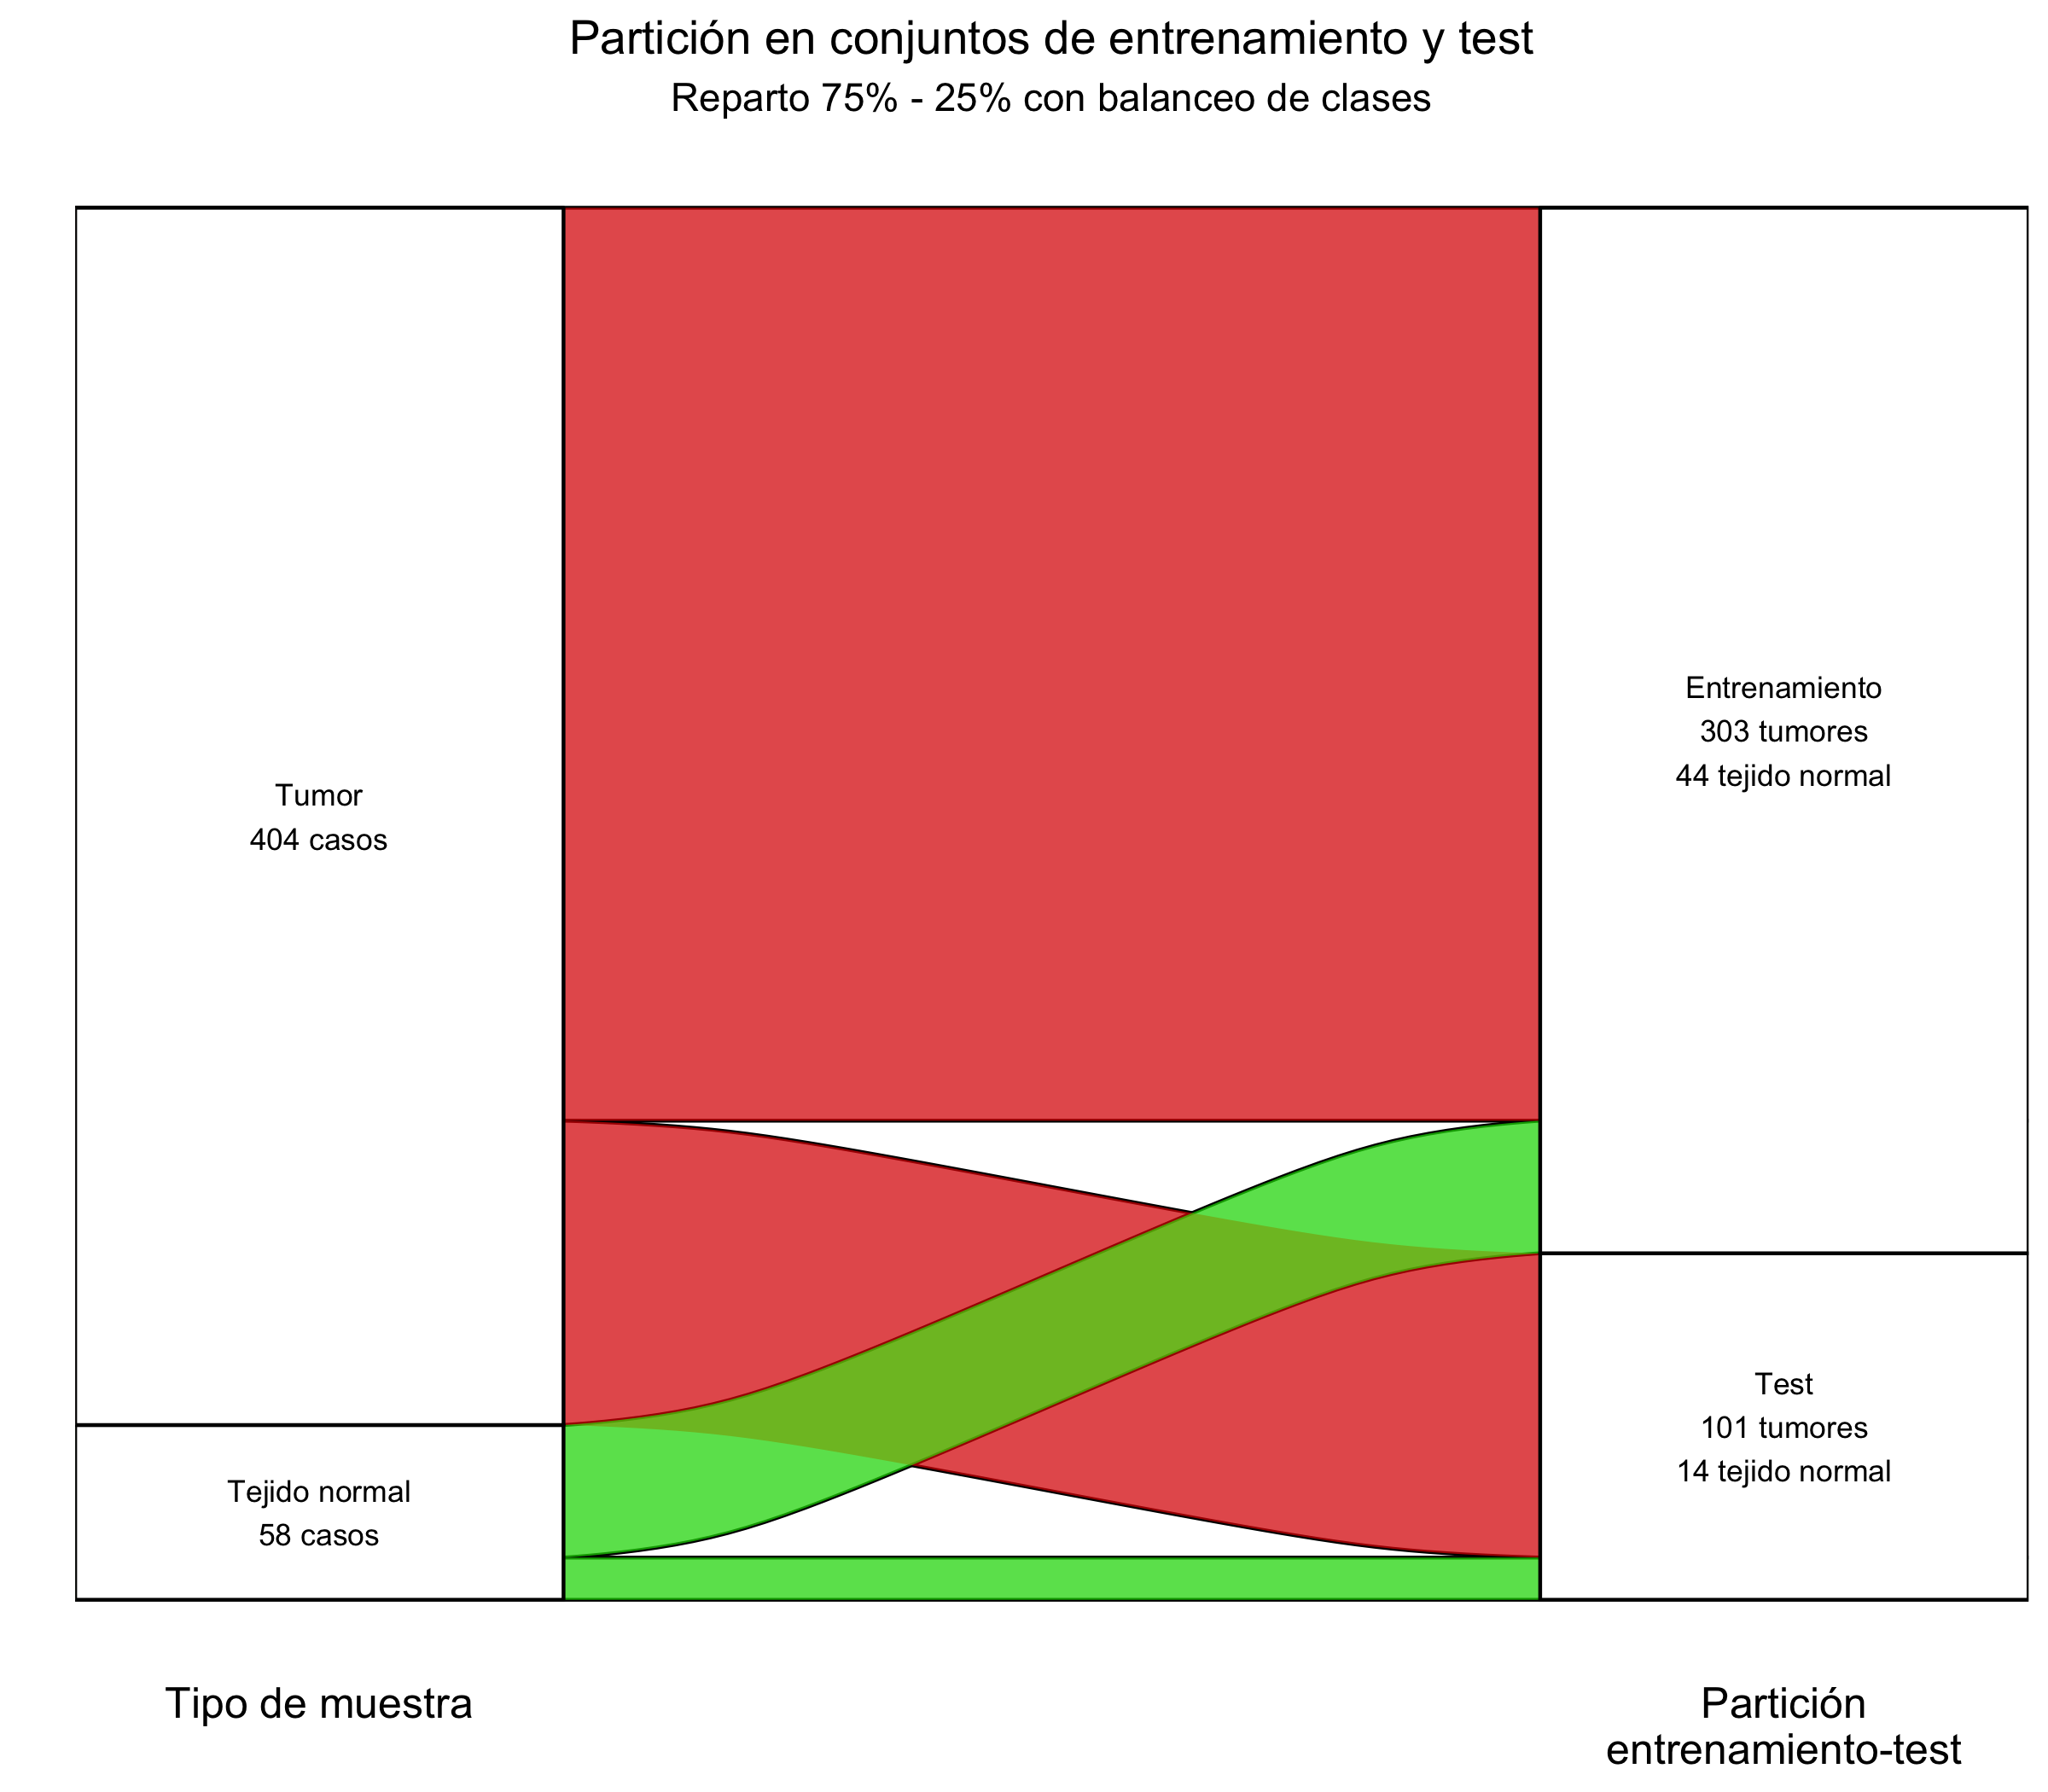
\includegraphics[width=1\textwidth]{figuras/higado_biclase_sankey.png} \\
\end{center}

\newpage
\subsubsection{SVM}

\textbf{\textcolor{red}{Figura XX}}. F1-Score con SVM en cada fold según método de selección de características y número de genes usados.
\begin{center}
	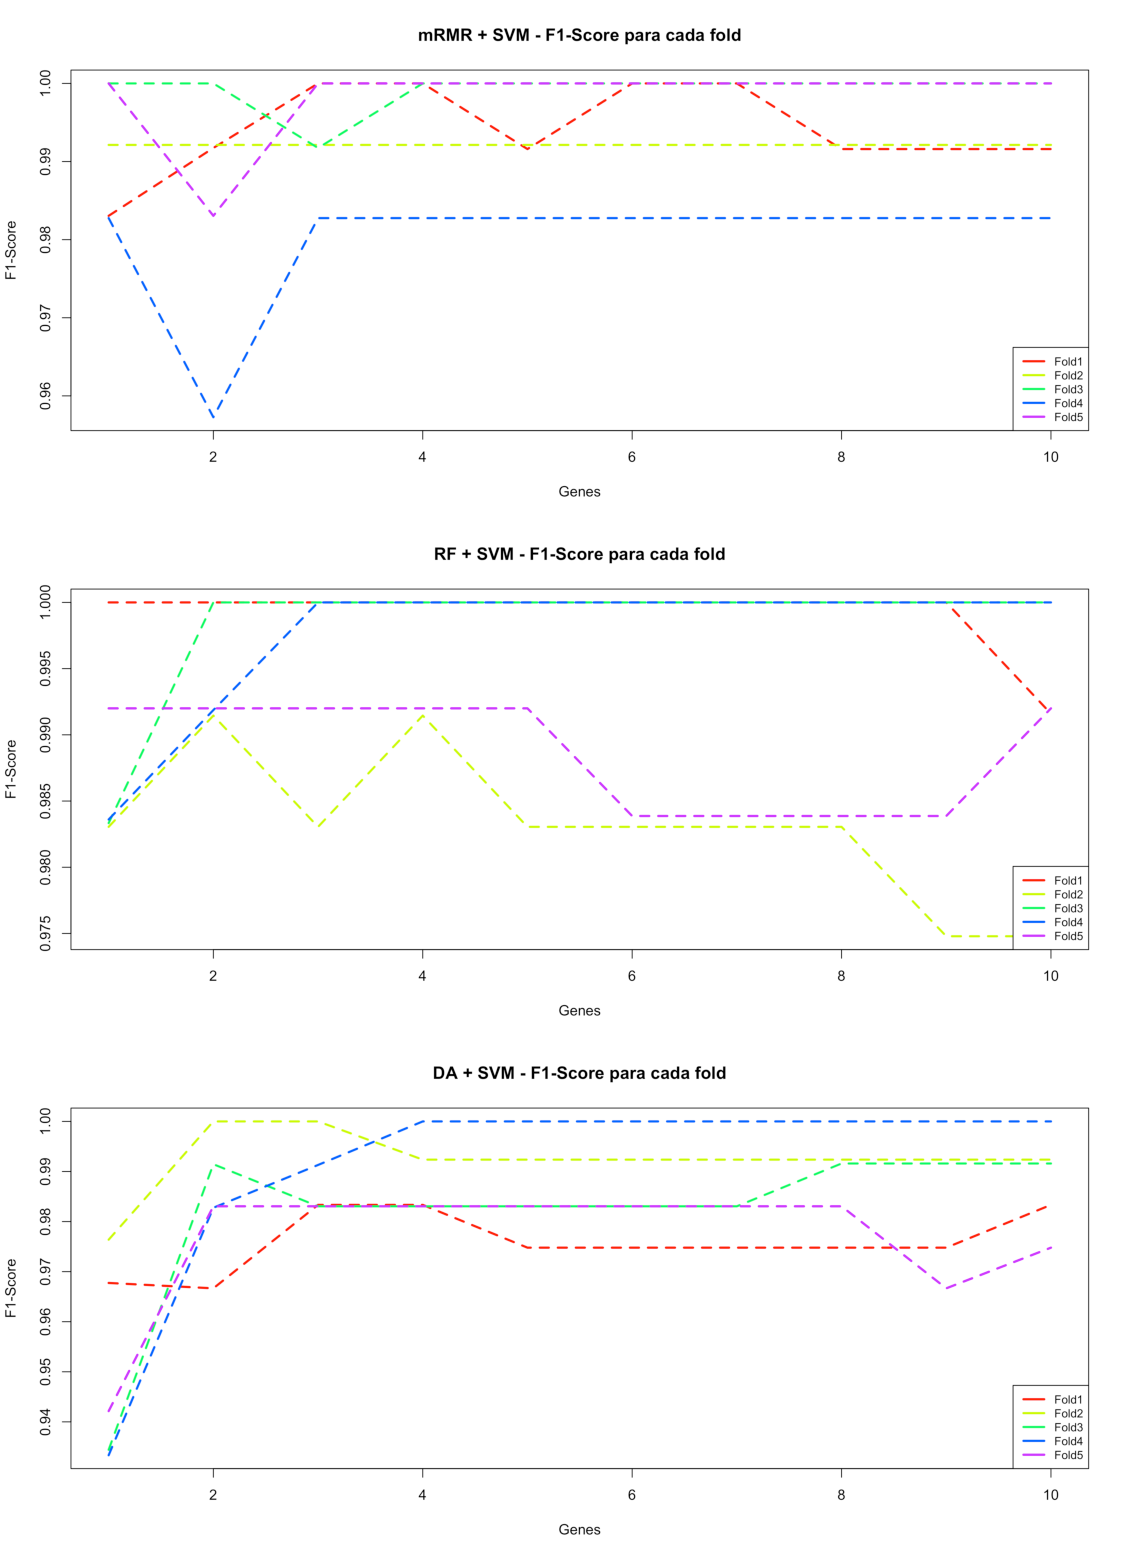
\includegraphics[width=.95\textwidth]{figuras/higado_biclase_folds_f1_svm.pdf} \\
\end{center}

\newpage
\textbf{\textcolor{red}{Figura XX}}. Precisión con SVM en cada fold según método de selección de características y número de genes usados.
\begin{center}
	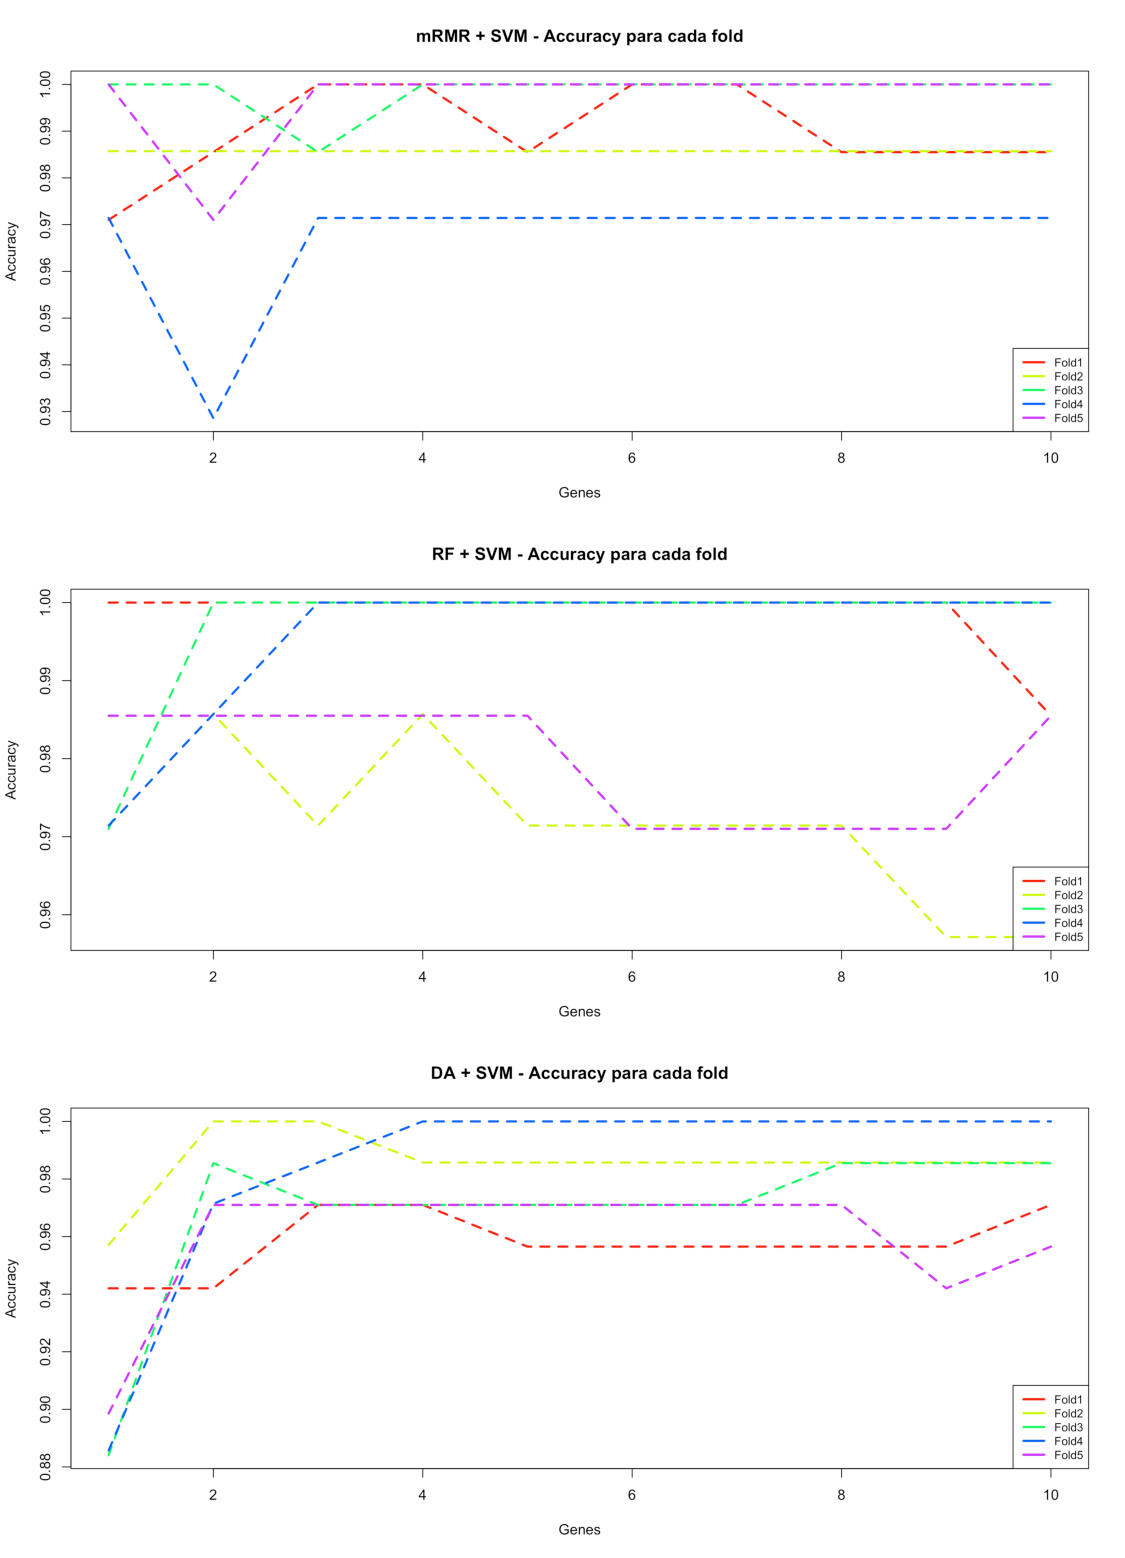
\includegraphics[width=.95\textwidth]{figuras/higado_biclase_folds_acc_svm.pdf} \\
\end{center}

\newpage
\textbf{\textcolor{red}{Figura XX}}. Mapa de calor con valores de F1-Score, precisión, sensibilidad y especificidad de SVM según método de selección de características y número de genes usados.
\begin{center}
	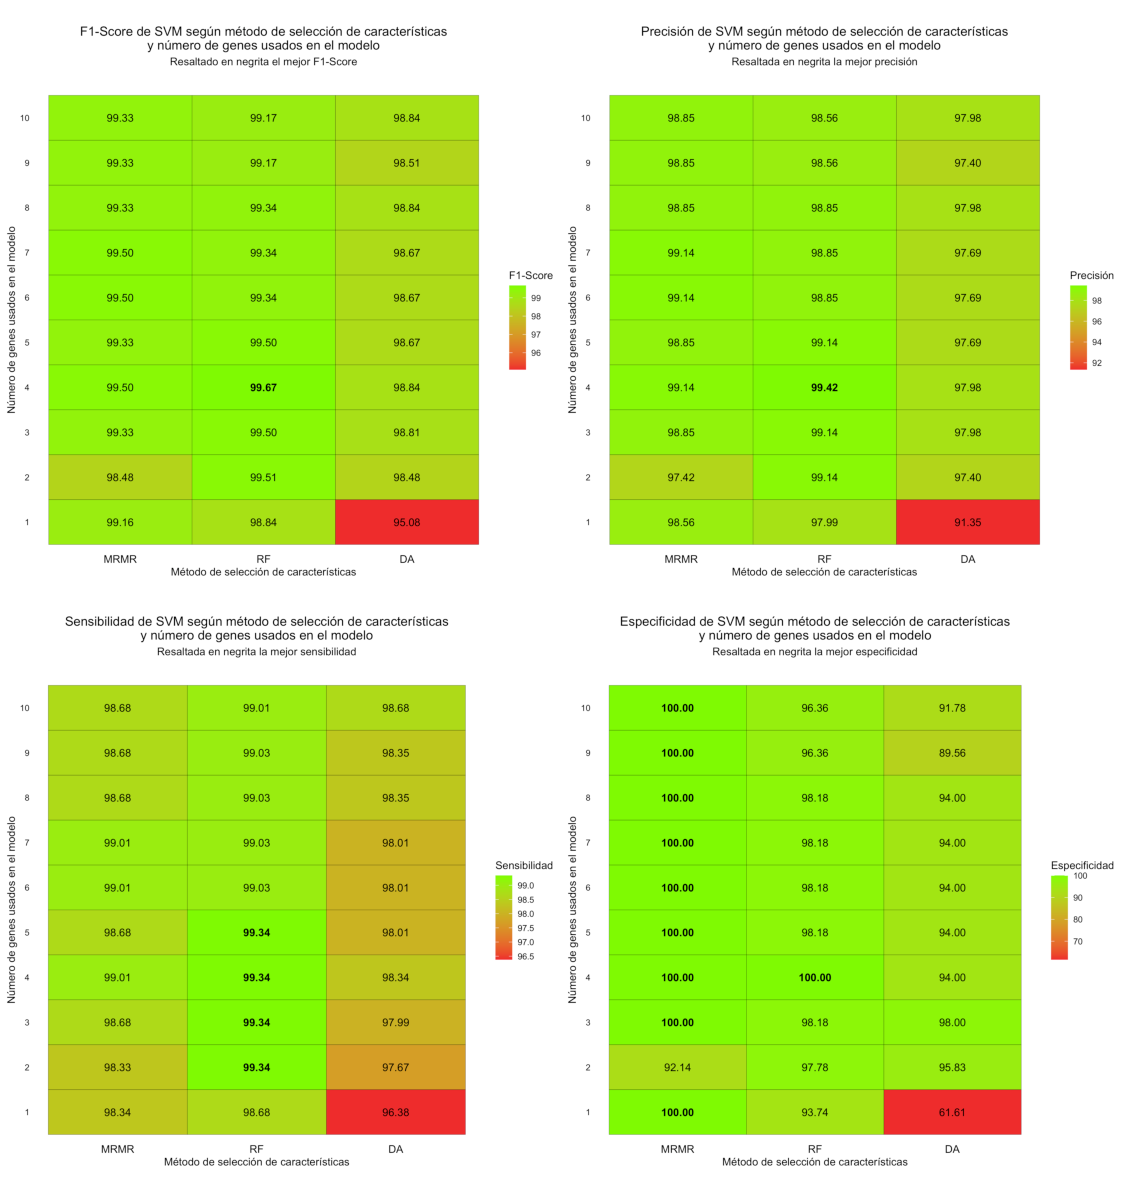
\includegraphics[width=1\textwidth]{figuras/higado_biclase_heatmap_svm.pdf} \\
\end{center}

\newpage
\subsubsection{RF}

\textbf{\textcolor{red}{Figura XX}}. F1-Score con RF en cada fold según método de selección de características y número de genes usados.
\begin{center}
	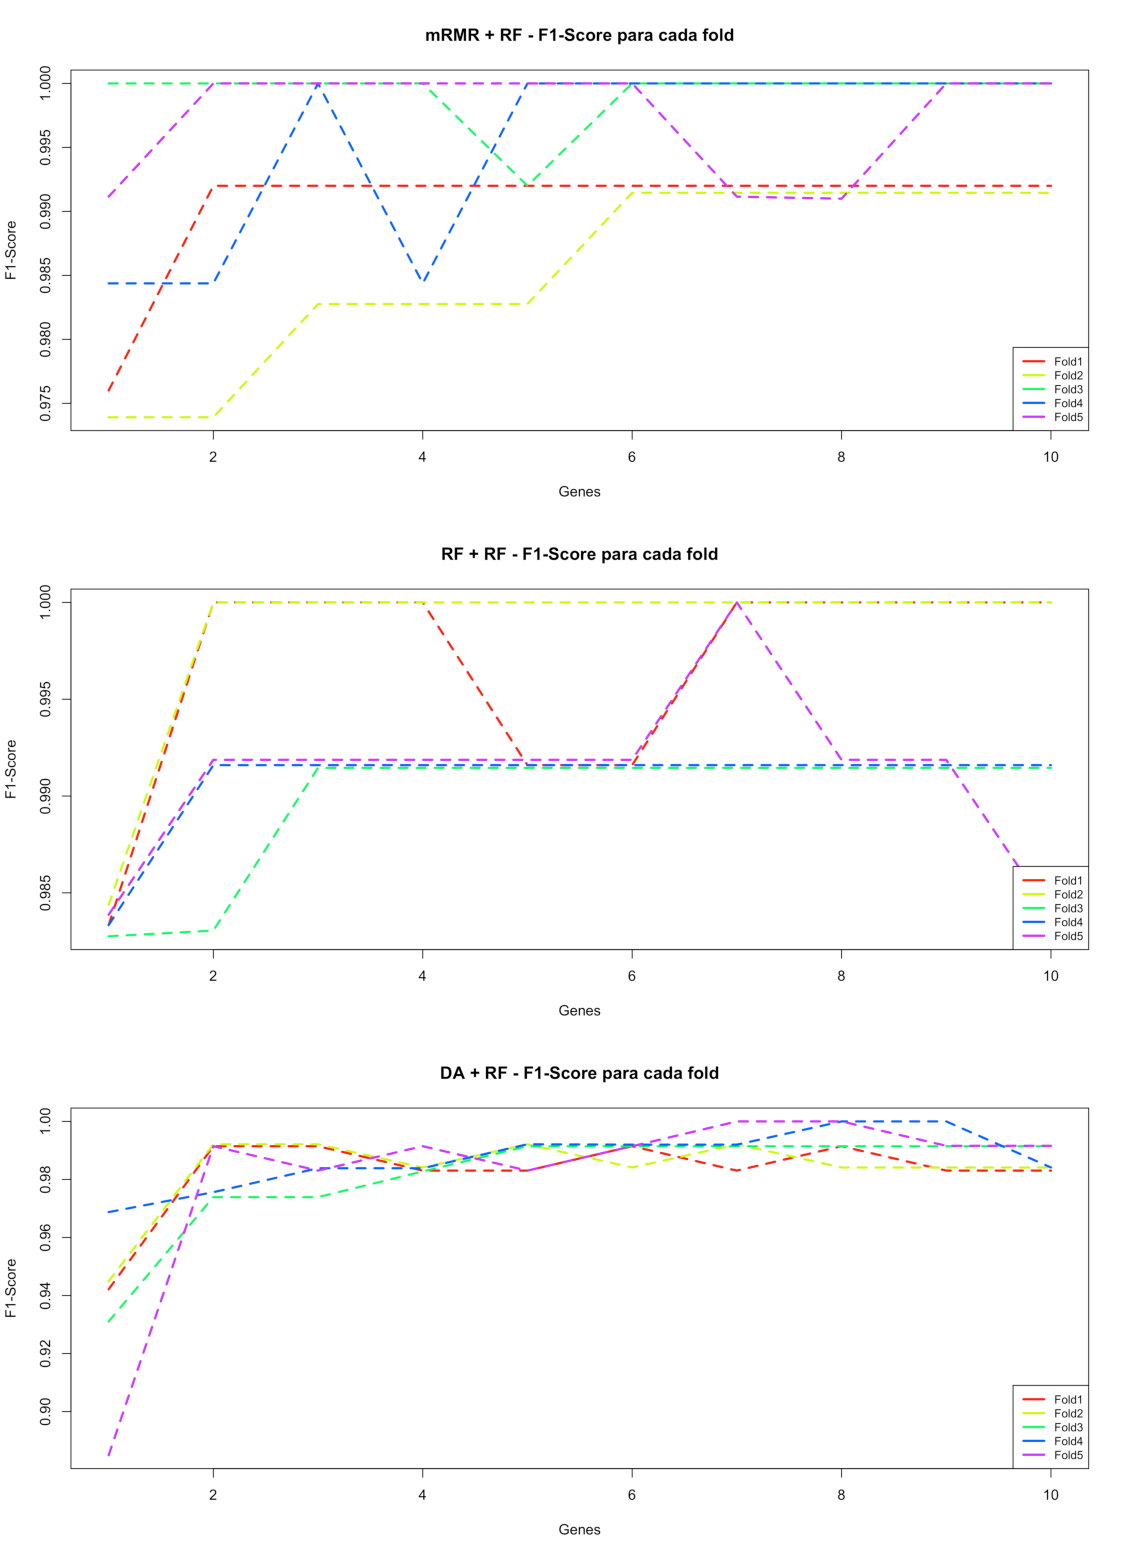
\includegraphics[width=.95\textwidth]{figuras/higado_biclase_folds_f1_rf.pdf} \\
\end{center}

\newpage
\textbf{\textcolor{red}{Figura XX}}. Precisión con RF en cada fold según método de selección de características y número de genes usados.
\begin{center}
	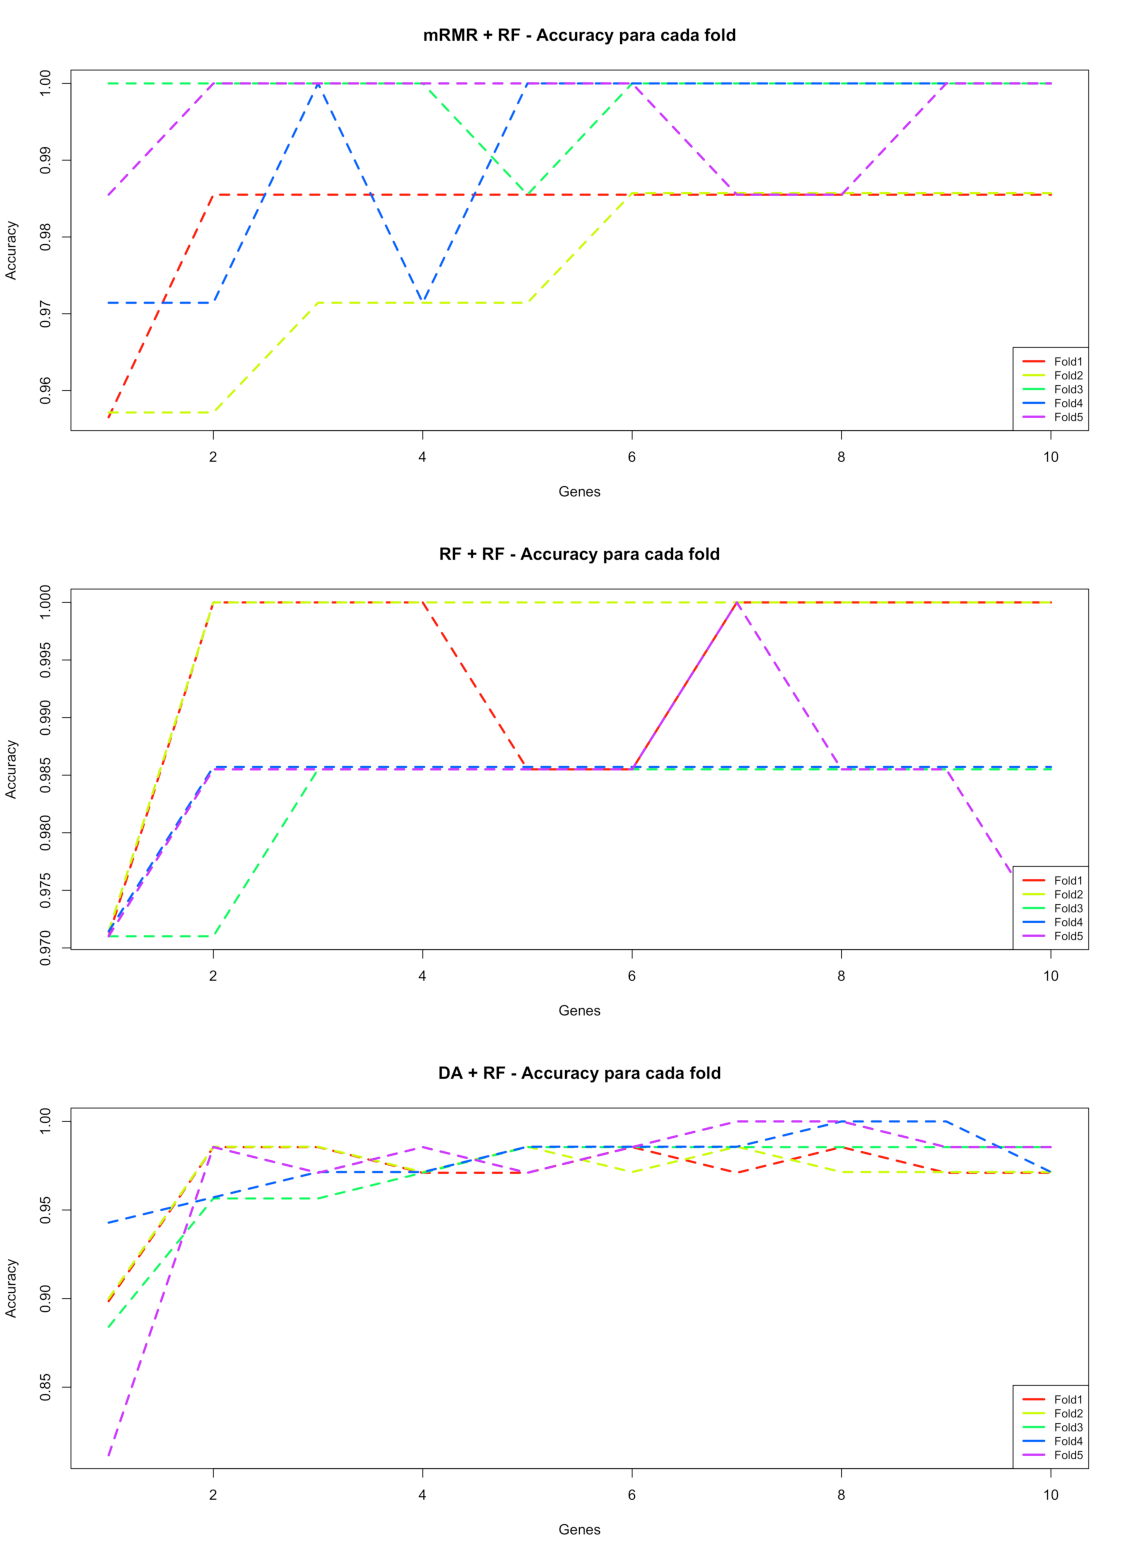
\includegraphics[width=.95\textwidth]{figuras/higado_biclase_folds_acc_rf.pdf} \\
\end{center}

\newpage
\textbf{\textcolor{red}{Figura XX}}. Mapa de calor con valores de F1-Score, precisión, sensibilidad y especificidad de RF según método de selección de características y número de genes usados.
\begin{center}
	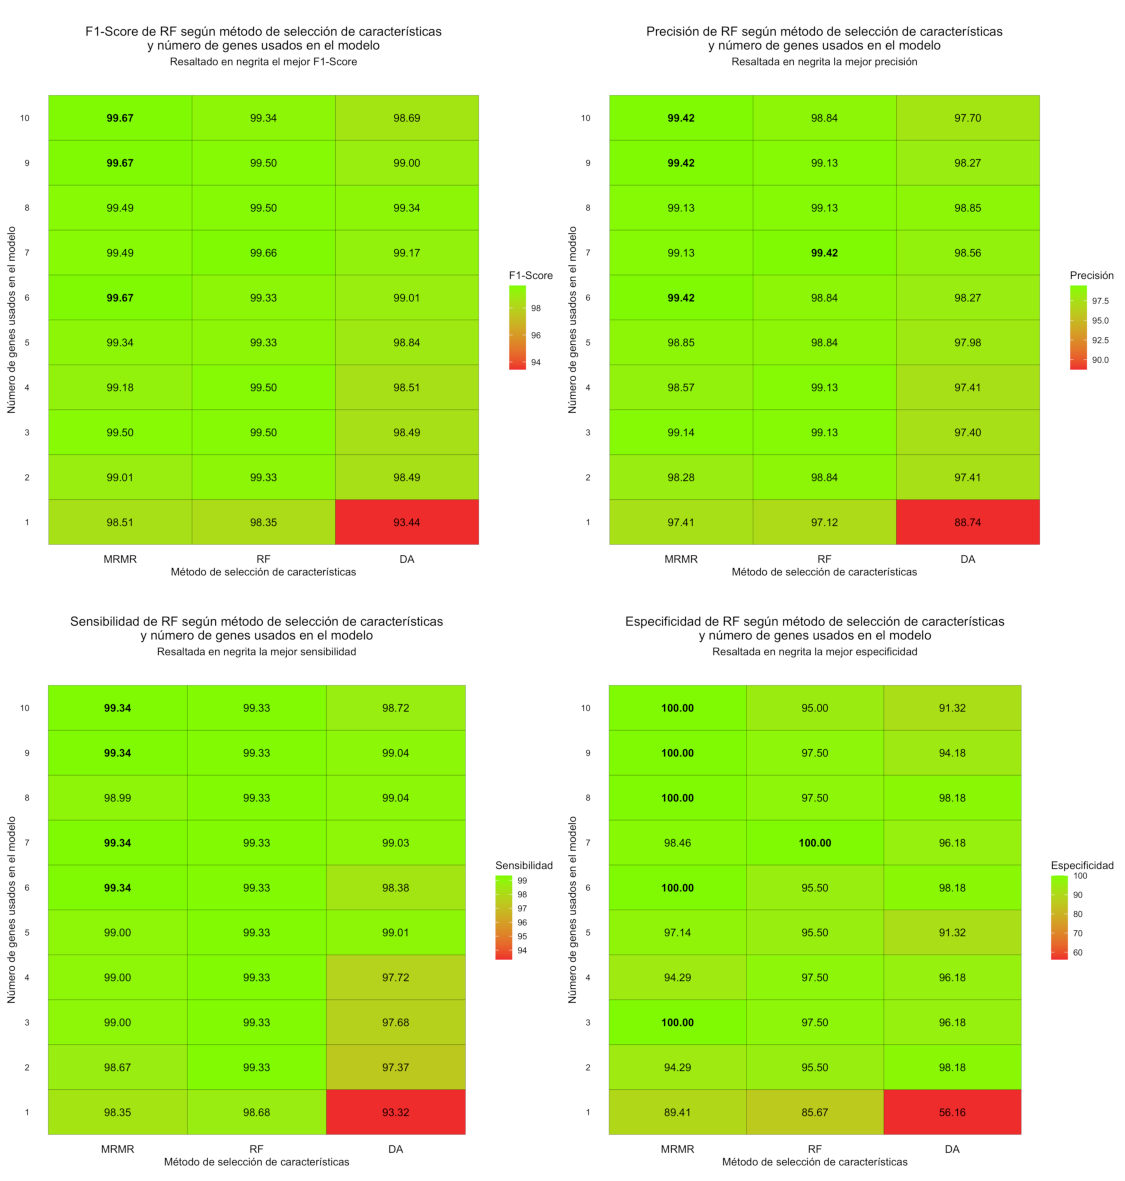
\includegraphics[width=1\textwidth]{figuras/higado_biclase_heatmap_rf.pdf} \\
\end{center}

\newpage
\subsubsection{kNN}

\textbf{\textcolor{red}{Figura XX}}. F1-Score con kNN en cada fold según método de selección de características y número de genes usados.
\begin{center}
	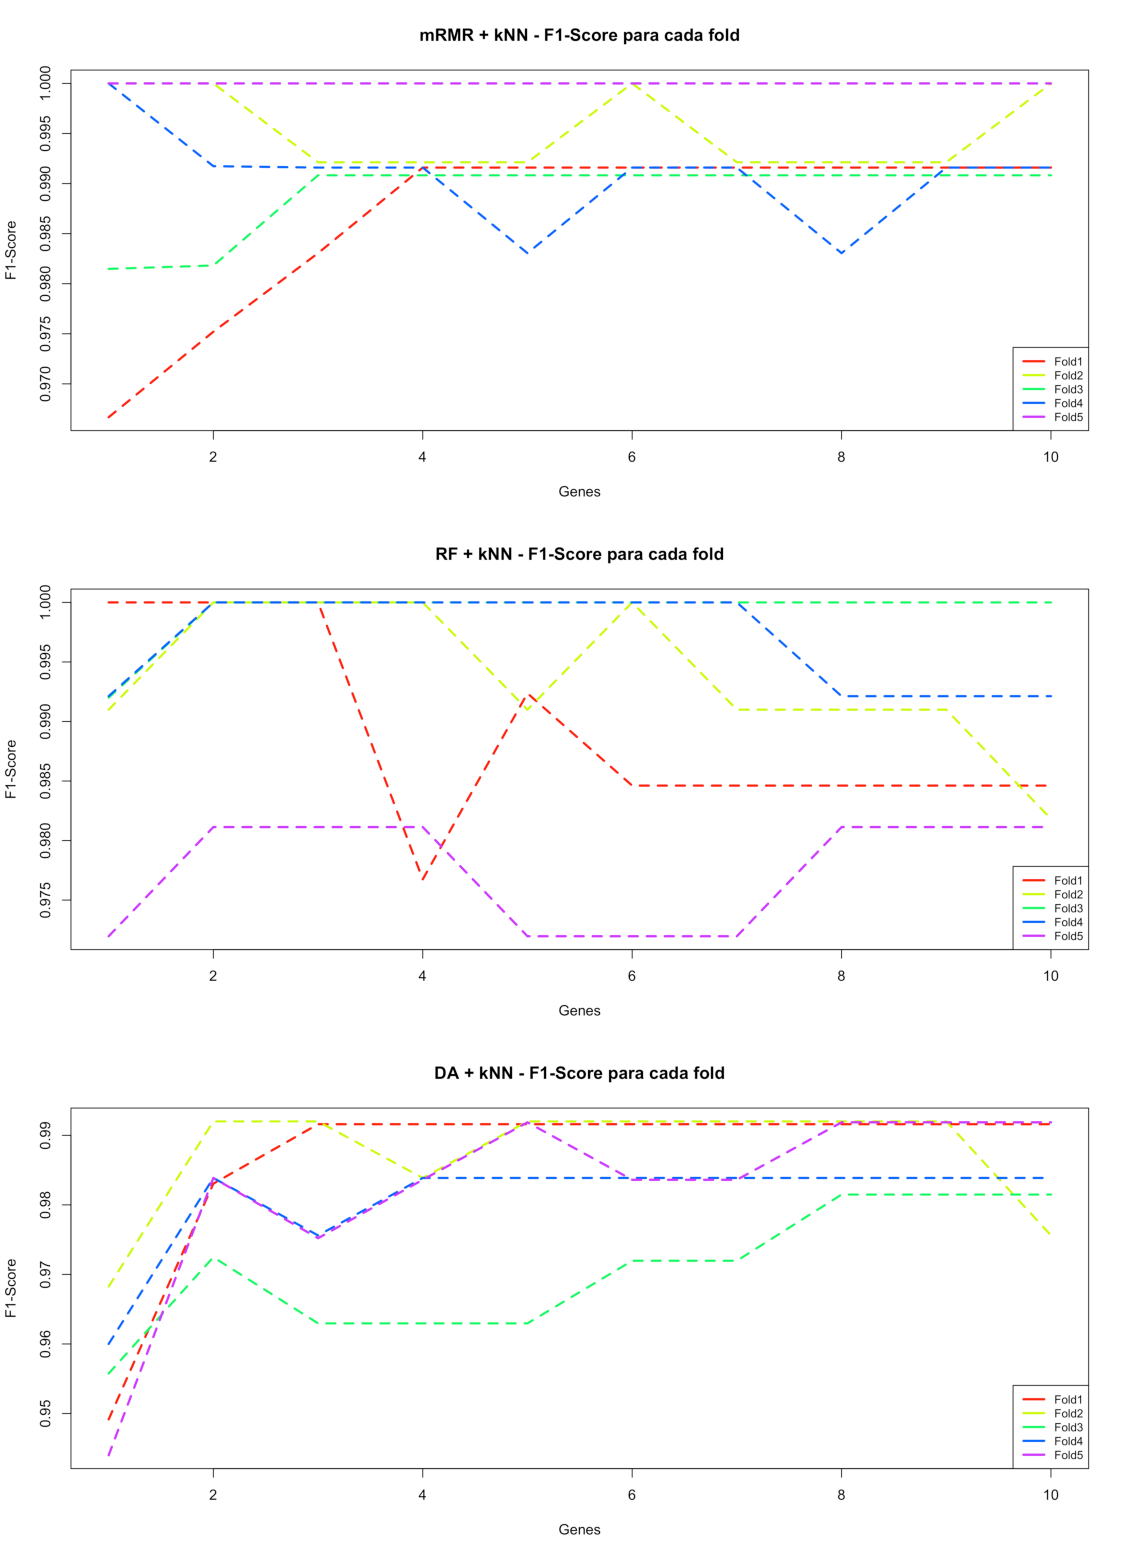
\includegraphics[width=.95\textwidth]{figuras/higado_biclase_folds_f1_knn.pdf} \\
\end{center}

\newpage
\textbf{\textcolor{red}{Figura XX}}. Precisión con kNN en cada fold según método de selección de características y número de genes usados.
\begin{center}
	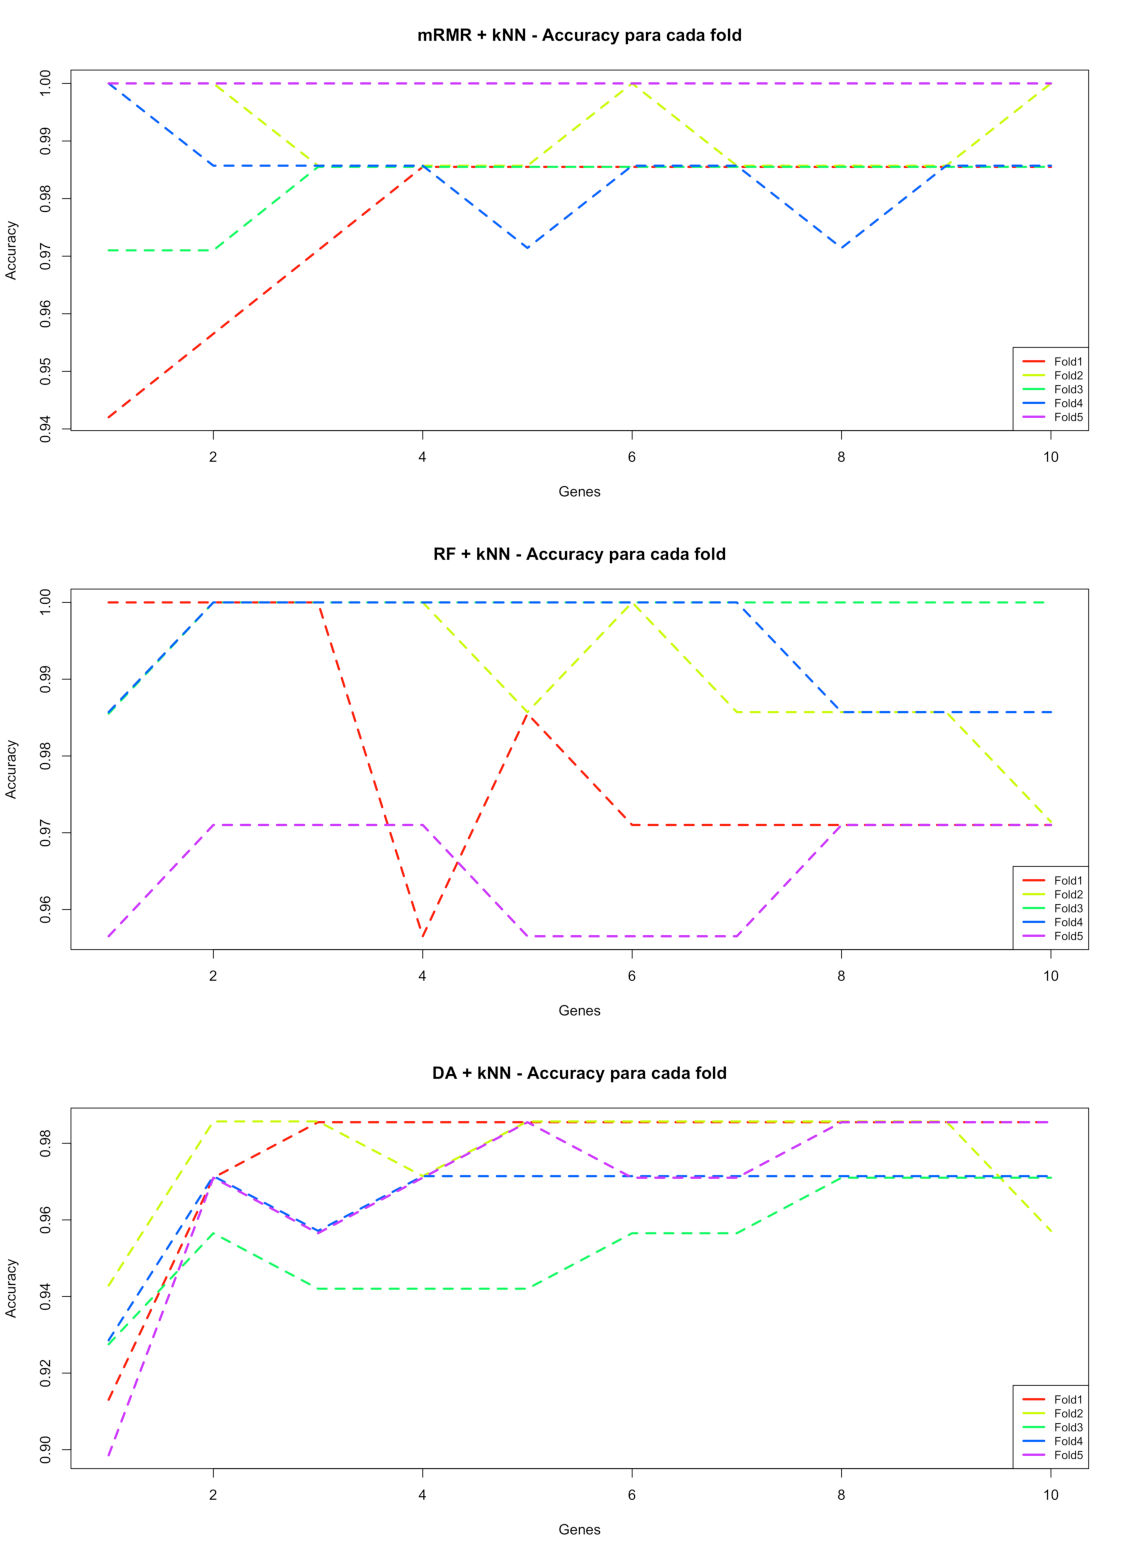
\includegraphics[width=.95\textwidth]{figuras/higado_biclase_folds_acc_knn.pdf} \\
\end{center}

\newpage
\textbf{\textcolor{red}{Figura XX}}. Mapa de calor con valores de F1-Score, precisión, sensibilidad y especificidad de kNN según método de selección de características y número de genes usados.
\begin{center}
	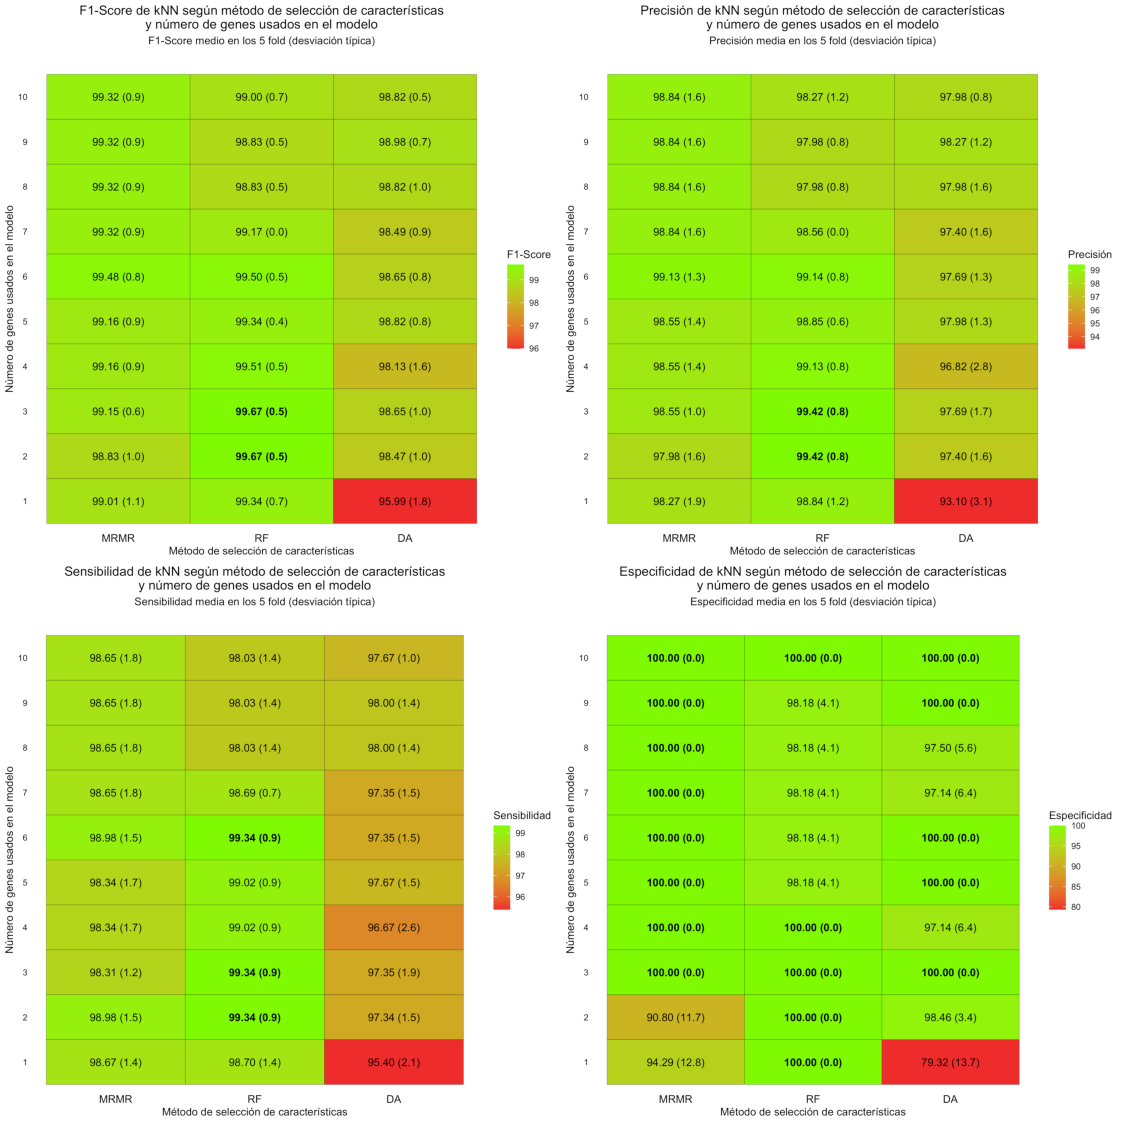
\includegraphics[width=1\textwidth]{figuras/higado_biclase_heatmap_knn.pdf} \\
\end{center}
\newpage

\subsection{Validación en test}

\section{Resultados de clasificación multiclase para cáncer de hígado}

El código completo del análisis se muestra en el fichero \texttt{analisis\_higado/\linebreak04\_analisis\_multiclase.R} del repositorio de GitHub asociado al trabajo \cite{Redondo-Sanchez2020}.\\

\section{Resultados de clasificación biclase para cáncer de colon-recto}

\textcolor{red}{Completar una vez esté depurado el análisis de cáncer de hígado.}

\section{Resultados de clasificación multiclase para cáncer de colon-recto}

\textcolor{red}{Completar una vez esté depurado el análisis de cáncer de hígado.}

\section{Conclusiones}

\textcolor{red}{Interpretar resultados con cautela: ver pág. 65 de \cite{CastilloSecilla2020} (referencias 77-79). Puede haber también con validación externa de los resultados.}\\

